\section{Wittgenstein’s Contribution to Inference: Meaning Without Model}

\subsection{Inference as Language Game}

Variational inference and concentration inequalities offer two complementary strategies for managing uncertainty. But both are grounded in formal systems: probabilistic models, cost functionals, KL divergences, and bounded random variables. They are powerful—but brittle. When the assumptions fail—such as mismatched support, improper priors, or unrealistic i.i.d. data—the whole apparatus begins to stutter.

This brittleness reveals a deeper philosophical tension. Logical systems, like those underlying KL divergence or tail bounds, operate through axioms and fixed semantics. Meaning is assigned via truth-values across hypothetical worlds—a structure reminiscent of possible world semantics.

Wittgenstein’s later philosophy offers a contrasting methodology—not mathematical, but contextual. In his framework of language games, meaning doesn’t arise from truth conditions in abstract models, but from use: from how words are employed within specific forms of life. This view recasts inference not as the pursuit of objective truth, but as the coordination of practice—how agents act, speak, and interpret within shared social environments.

In modeling complex phenomena—like elections, ideology formation, or cultural dynamics—Wittgenstein’s emphasis on context, interaction, and evolving norms provides a lens for capturing meaning as emergent and adaptive. It shifts the modeling goal from identifying universal truths to tracing locally coherent usage patterns.

This is where grounded theory enters the picture. Instead of forcing data into predefined categories, it seeks conceptual saturation: the point at which further observation adds no new patterns of meaning. In a world where truth is socially constructed, that’s not a limitation—it’s the finish line. When the language stabilizes through repeated use, when agents begin to play the same game, you don’t need more inference. You’ve reached shared meaning.

This complements variational methods, which seek not truth but usefulness—models that compress, explain, or generalize well, even if they're not ``correct'' in the absolute sense.

In the variational view:
\begin{itemize}
    \item Beliefs are encoded as distributions.
    \item Actions arise as optimal inferences under constraints.
\end{itemize}

In Wittgenstein’s world:
\begin{itemize}
    \item Beliefs are not ``internal representations'' but rules for participating in a form of life.
    \item Meaning is not reducible to a single trajectory or truth function—it is a \textbf{social regularity of use}.
\end{itemize}

This provides a foundation for interpreting concentration inequalities as guardrails for action in an uncertain world. They don’t aim to be universal laws, but context-sensitive heuristics. In Wittgenstein’s terms, they are tools for navigating uncertainty-laden language games where you don’t know the full game board, but still need to make a move.

\begin{quote}
``Don’t ask for the meaning, ask for the use.'' \\
\hfill — \textit{Wittgenstein, Philosophical Investigations}
\end{quote}

\subsection{A Wittgensteinian Agent-Based Model: Context, Feedback, and Lebesgue Integration}

Here, we sketch a Wittgensteinian approach to agent-based modeling that reflects the logic of language games and social feedback in continuous settings. Rather than assuming static beliefs or fixed voter categories, this simulation models the dynamic co-creation of meaning and influence across a network of agents embedded in contextual communication environments.

The simulation aims to capture how political beliefs form and evolve—not simply as rational updates from new information, but as emergent patterns of interpretation shaped by who is speaking, where they are speaking, and how others react. This approach treats language as situated practice, not just symbolic code.

In concrete terms, the simulation tracks how political ideas (like a candidate’s slogan) spread and transform meaning across social contexts (like subreddits, text chains, or media bubbles). It measures how agents interpret those ideas, influence one another, and gradually cluster into interpretive communities. The end result is not a probability of voting outcomes, but a real-time map of belief flow, semantic shift, and ideological alignment.

By treating meaning as emergent from use—rather than assigned from above—this model mirrors the logic of Wittgenstein’s later philosophy. It provides a new computational lens for studying elections: not as static outcomes, but as living ecologies of language, interaction, and persuasion.


\subsection{Agents, Contexts, and Meaning Spaces}

Let \( \mathcal{A} \) be a set of agents, indexed by \( a \in \mathcal{A} \), and let \( \mathcal{C} \) be the set of linguistic or cultural contexts in which these agents operate (e.g., social media threads, group chats, news sources). Let \( \mathcal{L} \) be the space of utterances, signals, or symbols exchanged between agents.

\paragraph{Agents \( \mathcal{A} \):}
The set \( \mathcal{A} \) represents individual participants in a sociolinguistic ecosystem—users in a networked system, political actors, voters, or even AI bots. Each agent \( a \in \mathcal{A} \) has an internal belief system, behavioral tendencies, and a propensity to generate or react to information. In the context of a political campaign, these agents could be voters segmented by geography, ideology, or demographics. In a Wittgensteinian sense, they do not act as atomic entities but as players embedded in overlapping “language games,” forming part of a socially constructed web of meaning.

\paragraph{Contexts \( \mathcal{C} \):}
The space \( \mathcal{C} \) is where meaning is born. It denotes the environments—both physical and virtual—that provide interpretive scaffolding for communication. Think of Reddit threads, WhatsApp group chats, or even a family dinner table. These contexts provide not only a medium for signal exchange but also define the rules of interpretation. For example, the phrase “fake news” may carry ridicule in one subculture and genuine concern in another. In this modeling framework, \( \mathcal{C} \) determines how utterances are framed, understood, and acted upon, much like how Wittgenstein emphasized that meaning arises from use within a form of life.

\paragraph{Linguistic and Symbolic Space \( \mathcal{L} \):}
The domain \( \mathcal{L} \) consists of all utterances, emojis, hashtags, visual memes, political slogans, and even silence—that is, any signal exchanged between agents. Each element \( \ell \in \mathcal{L} \) gains its meaning only within a context \( c \in \mathcal{C} \), and in relation to the communicative norms of a particular agent \( a \in \mathcal{A} \). For instance, the emoji “🔥” might signal enthusiasm in a music fan forum but could indicate danger in a wildfire alert group. Rather than treating \( \mathcal{L} \) as fixed semantic tokens, this model embraces language as fluid, polysemous, and rooted in socially situated interpretation—a direct echo of Wittgenstein’s notion of “family resemblance” among words rather than strict definitions.

Each agent \( a \) has a context-dependent meaning function:
\[
M_a: \mathcal{L} \times \mathcal{C} \to [0,1]
\]
which represents how that agent interprets a linguistic token within a given context. These meanings are not fixed—they evolve as agents interact.

\paragraph{Contextual Meaning Function \( M_a \):}
Each agent \( a \in \mathcal{A} \) is equipped with a personal, evolving function
\[
M_a: \mathcal{L} \times \mathcal{C} \to [0,1]
\]
which maps pairs of linguistic signals and contexts to a value representing the strength, salience, or alignment of meaning for that agent. The output is not an absolute truth or categorical interpretation—it is a probabilistic, context-dependent valuation that reflects how that particular agent understands or reacts to a given symbol in a given setting.

\paragraph{Interpretation as Situated Inference:}
This formulation breaks with classical semantics. Instead of treating language as a fixed dictionary of terms, it assumes that interpretation is situated, historical, and dialogical. An agent’s meaning function changes as it encounters new contexts or as its interactions reshape prior associations.

\paragraph{Example:}
Suppose the signal is the hashtag “\#freedom” and the context is a conservative-leaning political subreddit. For agent \( a_1 \), who frequently engages with libertarian discourse, we might have:
\[
M_{a_1}(\text{\#freedom}, \text{r/Conservative}) = 0.92
\]
indicating a strong positive identification and shared semantic alignment.

Meanwhile, agent \( a_2 \), who frequents social justice forums and is skeptical of the co-option of “freedom” in certain ideological frames, might have:
\[
M_{a_2}(\text{\#freedom}, \text{r/Conservative}) = 0.35
\]
reflecting interpretive dissonance or partial rejection of the term’s usage in that context.

\paragraph{Wittgensteinian Interpretation:}
These functions illustrate how language use is embedded in a “form of life.” The same symbol does not carry a single essence—it gains its pragmatic force from how it is used, by whom, and in what setting. Over time, as \( a_1 \) and \( a_2 \) interact or migrate across contexts, their respective \( M_a \) functions may shift. This models language not as code, but as adaptive social behavior—rooted in practice, revised through interaction.

\subsection{Continuous Belief Evolution via Feedback}

We define a feedback kernel \( K: \mathcal{A} \times \mathcal{A} \times \mathcal{C} \to \mathbb{R}_+ \), encoding how much agent \( a' \) influences agent \( a \) in context \( c \). Then, agent \( a \)'s belief over an idea or candidate \( \theta \in \Theta \) evolves according to:
\[
B_a(\theta) = \int_{\mathcal{A}} \int_{\mathcal{C}} K(a, a', c) \cdot M_{a'}(\ell_{\theta}, c) \, d\mu(a') \, d\nu(c)
\]
where \( \ell_{\theta} \in \mathcal{L} \) is a linguistic representation of \( \theta \), and \( \mu \), \( \nu \) are measures over agents and contexts respectively. This is a continuous version of influence modeling—akin to a social field equation.

\paragraph{The Feedback Kernel \( K(a, a', c) \):}
We define a \textbf{feedback kernel}
\[
K: \mathcal{A} \times \mathcal{A} \times \mathcal{C} \to \mathbb{R}_+
\]
which measures how much influence agent \( a' \) has on agent \( a \) within a particular context \( c \). This kernel encodes the strength, direction, and situational relevance of social interaction. It serves as a kind of "coupling coefficient" in the social field—quantifying how beliefs propagate across networks, platforms, and conversational spaces.

\paragraph{Belief as Weighted Social Integration:}
Given an idea or political candidate \( \theta \in \Theta \), represented by some linguistic symbol \( \ell_\theta \in \mathcal{L} \), we model agent \( a \)'s belief as:
\[
B_a(\theta) = \int_{\mathcal{A}} \int_{\mathcal{C}} K(a, a', c) \cdot M_{a'}(\ell_{\theta}, c) \, d\mu(a') \, d\nu(c)
\]

Here:
\begin{itemize}
    \item \( M_{a'}(\ell_{\theta}, c) \) encodes how strongly agent \( a' \) endorses or interprets \( \theta \) in context \( c \),
    \item \( K(a, a', c) \) tells us how much agent \( a \) listens to \( a' \) in that context,
    \item \( \mu \) is a measure over agents (e.g., weighting influence by popularity or proximity),
    \item \( \nu \) is a measure over contexts (e.g., emphasizing recent or emotionally salient situations).
\end{itemize}

\paragraph{Example: Election Influence Modeling}

Imagine a 2028 U.S. presidential election scenario:
\begin{itemize}
    \item Agent \( a \) is a politically undecided Twitter user.
    \item Agent \( a' \) is a viral political influencer with high contextual relevance in a trending debate (context \( c = \text{``climate policy thread''} \)).
    \item \( \ell_\theta = \text{\#NetZeroNow} \), a slogan used by candidate \( \theta \).
\end{itemize}

If:
\[
M_{a'}(\text{\#NetZeroNow}, c) = 0.93 \quad \text{(very favorable)}
\]
and:
\[
K(a, a', c) = 0.82 \quad \text{(agent $a$ frequently retweets $a'$ in this context)},
\]
then the product \( K(a, a', c) \cdot M_{a'}(\ell_{\theta}, c) \) makes a significant contribution to \( B_a(\theta) \).

Now suppose that across many agents and contexts, we integrate all such weighted endorsements. The result is a \textit{social field theory} of belief formation—an elegant generalization of influence maximization, grounded in the language and context-dependent understanding of symbols.

\paragraph{Why KL Divergence Fails Here:}
Traditional divergence-based methods (e.g., minimizing \( \mathrm{KL}(q \| p) \)) assume fixed distributions over predefined outcomes. But in this setting:
\begin{itemize}
    \item The \textit{support} of belief evolves through interaction.
    \item Meanings are \textit{not fixed}, but change with use (\`a la Wittgenstein).
    \item Influence is not global or stationary—it is \textit{local}, contextual, and relational.
\end{itemize}

This framework better models what Cambridge Analytica allegedly exploited: language-game sensitive, context-aware feedback systems that nudge agents by shaping meaning over time.

\paragraph{Philosophical Connection:}
Wittgenstein argued that the meaning of a word is its use in a particular life-form. Here, we extend that into a formalism: beliefs are not just updated through raw probabilities, but through \emph{contextual alignments of meaning and influence}, integrated over continuous social and linguistic spaces.

\begin{quote}
    In this view, every belief is a contextual echo—shaped by who said it, where they said it, and how others interpreted it.
\end{quote}


\begin{figure}[H]
    \centering
    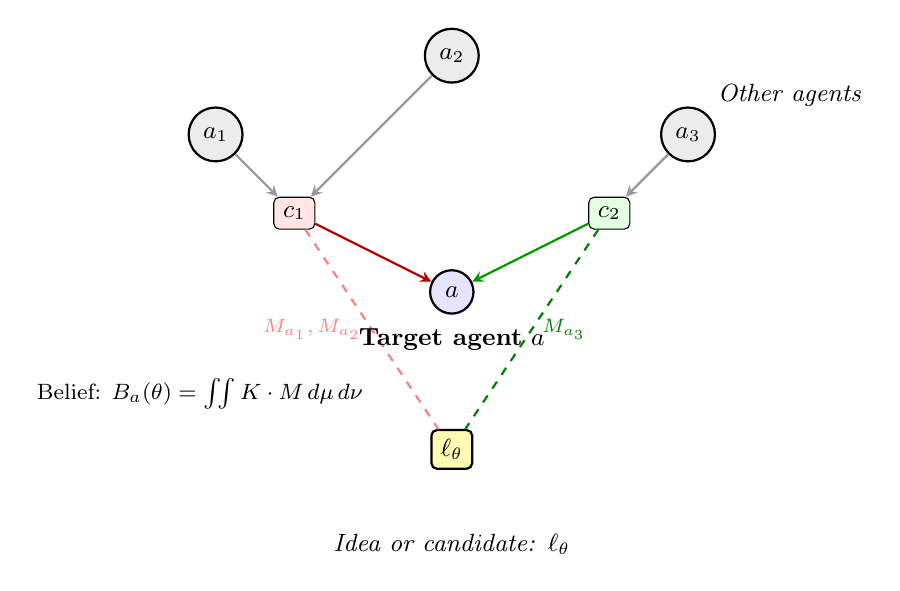
\begin{tikzpicture}[scale=1, every node/.style={font=\small}, node distance=1.8cm, >=stealth]
    
    % Agent nodes
    \node[circle, draw=black, fill=blue!10, thick] (A) at (0,0) {\(a\)};
    \node[circle, draw=black, fill=gray!15, thick] (A1) at (-3,2) {\(a_1\)};
    \node[circle, draw=black, fill=gray!15, thick] (A2) at (0,3) {\(a_2\)};
    \node[circle, draw=black, fill=gray!15, thick] (A3) at (3,2) {\(a_3\)};
    
    % Context nodes
    \node[rectangle, draw=black, fill=red!10, rounded corners=2pt] (C1) at (-2,1) {\(c_1\)};
    \node[rectangle, draw=black, fill=green!10, rounded corners=2pt] (C2) at (2,1) {\(c_2\)};
    
    % Utterance
    \node[rectangle, fill=yellow!30, draw=black, thick, rounded corners=2pt] (L) at (0,-2) {\(\ell_{\theta}\)};
    
    % Edges from A1, A2, A3 to C1, C2
    \draw[->, thick, gray!80] (A1) -- (C1);
    \draw[->, thick, gray!80] (A2) -- (C1);
    \draw[->, thick, gray!80] (A3) -- (C2);
    
    % Edges from contexts to A
    \draw[->, thick, red!70!black] (C1) -- (A);
    \draw[->, thick, green!60!black] (C2) -- (A);
    
    % Dashed lines from context to utterance meaning
    \draw[dashed, thick, red!50] (C1) -- (L) node[midway, left, font=\scriptsize] {\(M_{a_1}, M_{a_2}\)};
    \draw[dashed, thick, green!50!black] (C2) -- (L) node[midway, right, font=\scriptsize] {\(M_{a_3}\)};
    
    % Annotations
    \node[align=center] at (0,-3.2) {\textit{Idea or candidate:} \( \ell_{\theta} \)};
    \node[align=center] at (0,-0.6) {\textbf{Target agent} \( a \)};
    \node[align=center] at (4.3,2.5) {\textit{Other agents}};
    \node[align=center, font=\footnotesize] at (-3.2,-1.3) {Belief: \( B_a(\theta) = \int\!\!\int K \cdot M \, d\mu\, d\nu \)};
    
    \end{tikzpicture}
    \caption{A continuous agent-based belief model: meanings \( M_{a'}(\ell_\theta, c) \) flow through contexts \( c \), modulated by influence weights \( K(a,a',c) \), and are integrated to update agent \( a \)'s belief over \( \theta \).}
\end{figure}


\subsection{Family Resemblances in Action}

Rather than assuming fixed taxonomies (e.g., voters \textit{for} or \textit{against} an issue), this model traces how clusters of agents come to form overlapping, non-essentialist groupings—a Wittgensteinian "family resemblance."

Let \( G \subset \mathcal{A} \) be such a grouping. We define the resemblance score between agents \( a, a' \in \mathcal{A} \) as:
\[
R(a, a') = \int_{\mathcal{C}} \int_{\mathcal{L}} |M_a(\ell, c) - M_{a'}(\ell, c)| \, d\lambda(\ell) \, d\nu(c)
\]

Agents with low mutual \( R(a, a') \) scores cluster into interpretive communities—not via top-down ontologies, but through shared practices and language use.

\paragraph{Qualitative Interpretation}

This formalism captures a subtle but powerful idea: \textbf{similarity doesn’t arise from fixed categories, but from shared patterns of use}.

Rather than trying to classify agents into neat ideological bins---say, “progressives” versus “conservatives,” or “pro” versus “anti”—this approach looks at how agents interpret the world across contexts. If two people consistently react to linguistic tokens (like political slogans, hashtags, or policy language) in similar ways across a range of conversations and cultural settings, they resemble each other in the Wittgensteinian sense. They’re not identical, and they don’t necessarily agree on everything, but they inhabit a similar interpretive world.

\subparagraph{Example 1: Online Discourse Clusters}

Suppose Agent \( a \) and Agent \( a' \) frequently comment on online news articles. One might be from New York, the other from California. One might support increased taxation for the rich; the other might oppose it. But both consistently interpret posts about “economic fairness,” “student debt,” or “public services” in similar ways—they upvote the same replies, engage with similar memes, or use similar phrases.

Their resemblance score \( R(a, a') \) is low because their interpretation functions \( M_a \) and \( M_{a'} \) yield similar outputs across shared linguistic and contextual environments. They are not part of a pre-labeled demographic—but they form a cluster nonetheless. They exhibit \textbf{family resemblance}: overlapping features without any single defining trait.

\subparagraph{Example 2: Voter Behavior Without Ideological Labels}

In an election, traditional polling might ask whether voters support Policy X. But two voters might both answer “yes” for different reasons—one sees it as economically beneficial, the other as morally justified. If we study only the “yes” response, we collapse them into a category that hides the nuanced differences in interpretation.

However, using the \( R(a, a') \) framework, we can trace how they interpret various linguistic signals—statements from politicians, news articles, community discussions—and detect whether their agreement on Policy X is part of a broader interpretive similarity, or just a local coincidence.

\subparagraph{Beyond Classification: Towards Emergent Taxonomy}

In essence, this model sidesteps the limitations of top-down ontologies. Instead of assuming that groups exist a priori, it lets the groupings \textbf{emerge from patterns of interpretation}. Shared understanding is not presumed; it is measured through how agents respond to meaning in context.

These clusters are dynamic and overlapping. An agent may resemble one group in economic discussions, another in cultural contexts, and neither in matters of science or religion. This fluidity reflects real human discourse far better than rigid classification schemes.

\begin{quote}
Just as family members may share a nose, a laugh, or a stubborn streak—but not all at once—agents in a sociolinguistic system may share interpretive traits without sharing a strict identity.
\end{quote}

This is the logic of \textbf{family resemblances}, rendered mathematically. And it provides a foundation for modeling real-world meaning, influence, and belief—not as abstract categories, but as emergent, context-sensitive patterns of use.



\subsection{Election Modeling as Language Ecology}

Traditional election models often rely on fixed features—demographics, polling data, past voting records—to predict outcomes as probabilistic point estimates. But in a Wittgensteinian framework, the emphasis shifts: rather than treating voters as predefined units with static preferences, we view them as participants in a dynamic ecology of language, context, and interaction.

This model treats elections not as isolated decisions, but as unfolding \textbf{language games}. Words like “freedom,” “security,” or “justice” do not carry fixed meanings; instead, their interpretations evolve as they are used in different cultural and conversational settings. For instance, the term “freedom” might evoke anti-tax sentiment in one region and pro-civil rights advocacy in another. What matters is not the word itself, but how it is used—by whom, in what context, and with what effect.

\textbf{Feedback loops} are a central feature of this ecology. When a major influencer endorses a candidate or a meme goes viral, it shifts the shared contexts \( \mathcal{C} \). This change in context feeds back into how agents interpret linguistic signals and reshape their beliefs. For example, a news spike around immigration policy may alter the meaning of “security” across a network, intensifying certain associations and dampening others. This is not a one-way broadcast but an evolving, interactive process.

From these interactions, voter identities do not simply reflect stable ideologies—they \textbf{emerge} through patterns of linguistic usage, social proximity, and interpretive similarity. Clusters form not from top-down labeling (e.g., “liberal” vs. “conservative”), but from bottom-up resemblances in how people respond to language and context. One agent may align with others on economic rhetoric, while diverging sharply on environmental discourse.

The result of this model is not a crisp probability distribution over voter outcomes. Instead, it yields a \textbf{social field}—a map of influence, alignment, and meaning. It captures how shared language forms, spreads, and adapts in real-time, revealing interpretive communities, semantic tipping points, and zones of ideological fluidity. 

Remarkably, this social field can be treated analogously to a mathematical field in the Dedekind sense. Just as Dedekind envisioned number fields as complete, ordered structures that support addition and multiplication, we can interpret the space of agent alignments and contextual meanings as a composable algebraic system. Influence can be aggregated, meaning differentials can be combined, and contextual shifts act like field automorphisms—preserving structure while transforming interpretation. This opens the door to rigorous mathematical analysis: defining continuity, convergence, and even topology over networks of belief. In this sense, political behavior becomes not just a social phenomenon, but a structured, algebraically navigable landscape.

\begin{quote}
In a Wittgensteinian world where truth is use and identity is practice, this model doesn’t just track voter behavior—it tracks how political reality itself is constituted through linguistic interaction. And that is closer to how elections actually unfold than any opinion poll.
\end{quote}

\subsection{Mathematical Formalization of the Social Field}

Let us now treat the social belief landscape as a structured algebraic system, drawing an analogy to the Dedekind-style notion of a \textbf{field} in algebraic number theory.

\subsubsection{1. Defining the Social Field}

Let \( \mathcal{F} \) denote the set of contextualized agent beliefs:
\[
\mathcal{F} := \left\{ B_a(\theta) \;\middle|\; a \in \mathcal{A},\; \theta \in \Theta \right\}
\]

Each element \( B_a(\theta) \in [0,1] \) represents the belief strength of agent \( a \) in idea or candidate \( \theta \), as defined by:
\[
B_a(\theta) = \int_{\mathcal{A}} \int_{\mathcal{C}} K(a, a', c) \cdot M_{a'}(\ell_\theta, c) \, d\mu(a') \, d\nu(c)
\]

\subsubsection{Field Operations: Belief Algebra}

We introduce two operations over \( \mathcal{F} \) analogous to addition and multiplication:

\begin{itemize}
    \item \textbf{Addition} (belief aggregation):
    \[
    (B_1 + B_2)(\theta) := \alpha \cdot B_1(\theta) + (1 - \alpha) \cdot B_2(\theta)
    \]
    for some \( \alpha \in [0,1] \), modeling a convex combination of agent beliefs.

    \item \textbf{Multiplication} (belief alignment or reinforcement):
    \[
    (B_1 \cdot B_2)(\theta) := B_1(\theta) \cdot B_2(\theta)
    \]
    This reflects joint endorsement or signal amplification.
\end{itemize}

With appropriate normalization and closure assumptions, \( \mathcal{F} \) becomes a commutative ring with identity, and can be embedded into a field-like structure under suitable constraints (e.g., excluding belief-zero divisors).

\subsubsection{Meaning Differentials and Distance}

Define a \textbf{meaning differential} between two agents as:
\[
\Delta_{a, a'} := \int_{\mathcal{C}} \int_{\mathcal{L}} \left| M_a(\ell, c) - M_{a'}(\ell, c) \right| \, d\lambda(\ell) \, d\nu(c)
\]

This induces a metric (or semi-metric) over the agent space, allowing us to study convergence, continuity, and connected components in interpretive space.

\subsubsection{Contextual Automorphisms}

Let \( \varphi: \mathcal{C} \to \mathcal{C} \) be a context-shifting transformation (e.g., a trending event, algorithmic feed update, or meme cascade).

We define the action of \( \varphi \) on belief fields as:
\[
\varphi^*(B_a)(\theta) := \int_{\mathcal{A}} \int_{\mathcal{C}} K(a, a', \varphi(c)) \cdot M_{a'}(\ell_\theta, \varphi(c)) \, d\mu(a') \, d\nu(c)
\]

If \( \varphi \) is invertible and structure-preserving (e.g., semantic relationships are maintained), then it plays the role of a \textbf{field automorphism}—analogous to symmetries in algebraic structures.

\subsubsection{Toward a Topology of Belief}

Using the metric \( \Delta_{a,a'} \), we may endow \( \mathcal{A} \) (or \( \mathcal{F} \)) with a topology. Open sets correspond to interpretive neighborhoods, and we can define:

\begin{itemize}
    \item \textbf{Continuity:} Belief functions \( B_a(\theta) \) are continuous under smooth variation of context and influence.
    \item \textbf{Convergence:} Belief states converge as agents interact over time.
    \item \textbf{Connectedness:} Communities of mutual understanding emerge as path-connected components in the interpretive space.
\end{itemize}

\subsubsection*{Conclusion: Political Epistemology as Algebraic Geometry}

The social field of belief, constructed through linguistic use and contextual interpretation, supports algebraic and topological analysis. Rather than reducing political dynamics to static distributions or binary choices, this framework models belief as a dynamic, structured object—evolving within a Wittgensteinian grammar of use, and navigable like a Dedekind field of meanings.




